\documentclass[a4paper,12pt,oneside]{book}
\usepackage[T1]{fontenc}                                      
\usepackage[utf8]{inputenc}                               
\usepackage[italian]{babel}
\usepackage{amsfonts}
\usepackage{amsthm}
\usepackage{amsmath,amssymb}
\usepackage{array}
\usepackage{arydshln}
\usepackage{braket}
\usepackage{blindtext}
\usepackage{calc}
\usepackage{cancel}
\usepackage{caption}
\usepackage{epsfig}
\usepackage{eucal}
\usepackage{fancyhdr}
\usepackage{geometry}
\usepackage{graphicx}
\usepackage{indentfirst}
\usepackage{hhline}
\usepackage{hyperref}
\hypersetup{
			colorlinks=true,
			linkcolor=black,
			anchorcolor=black,
			citecolor=black,
			urlcolor=black,
			pdftitle={Appunti di Meccanica Quantistica},
			pdfauthor={Vittorio Lubicz}
}

\usepackage{latexsym}
\usepackage{listings} 
\usepackage{longtable}
\usepackage{makeidx}
\usepackage{mathrsfs}
\usepackage{mathdots}
\usepackage{multirow}
\usepackage{nicefrac}
\usepackage{pdfpages}
\usepackage{physics}
\usepackage{setspace}
\usepackage{tikz}
\usepackage{tikz-3dplot}
\usepackage{textcomp}
\usepackage{titlesec,color}
\usepackage{vmargin}
\setpapersize{A4}
\setmarginsrb{35mm}{30mm}{35mm}{30mm}%
             {0mm}{10mm}{0mm}{10mm}



\definecolor{gray75}{gray}{0.75}
\newcommand{\hsp}{\hspace{20pt}}

\titleformat{\chapter}[hang]{\huge\bfseries}{\myfont{\textit{\large{\chaptername\hspace{1pt} \thechapter\hspace{3pt}}}}\textcolor{gray75}{$\mid$}\hspace{0.4cm}}{0pt}{\myfont{\huge\bfseries}}

\titleformat{\section}[hang]{\large\bfseries}{\myfont{\textit{\normalsize{\thesection\hspace{2pt}}}}\hspace{0.4cm}}{0pt}{\myfont{\Huge\bfseries}}

\titleformat{\subsection}[hang]{\large\bfseries}{\myfont{\textit{\small{\thesubsection\hspace{2pt}}}}\hspace{0.4cm}}{0pt}{\myfont{\huge\bfseries}}

\renewcommand{\chaptermark}[1]{\markboth{#1}{}}
\renewcommand{\sectionmark}[1]{\markright{#1}}
\newcommand*{\myfont}{\fontfamily{ppl}\selectfont}

\begin{document}

%*****************LAYOUT PAGINE**************************
\fancypagestyle{plain}{%
\fancyhf{} % cancella tutti i campi di  intestazione e pi\`e di pagina
\fancyfoot[C]{\bfseries \myfont{\thepage}} % tranne il centro
\renewcommand{\headrulewidth}{0pt}
\renewcommand{\footrulewidth}{0pt}}

\fancypagestyle{VS}{
\headheight = 15pt
\lhead[\myfont{\textit{\textbf{\thechapter\nouppercase{\leftmark}}}}]{\myfont{\textit{\textbf{\nouppercase{\leftmark}}}}}
\chead[]{}
\rhead[\myfont{\textbf{\thepage}}]{\myfont{\textbf{\thepage}}}

\lfoot[]{}
\cfoot[]{}
\rfoot[]{}
}
%*******************************************************



\pagestyle{VS}
\setcounter{chapter}{22}
\setcounter{page}{227}
\chapter[Effetto Stark]{Effetto Stark\footnote{G16; S5.1,5.2}}
Se un atomo viene sottoposto ad un campo elettrico esterno, i suoi livelli energetici cambiano. Questo fenomeno è detto \textbf{effetto Stark}.
Supporremo che il campo elettrico sia sufficientemente debole, perché l'energia addizionale ad esso dovuta sia piccola rispetto alle distanze fra i livelli energetici vicini dell'atomo. Allora per calcolare gli spostamenti dei livelli un un campo elettrico, si può ricorrere alla \textbf{teoria delle perturbazioni}.\\
Ci proponiamo di calcolare, facendo uso della teoria delle perturbazioni, le correzioni al primo ordine da apportare ai livelli energetici dell'\textbf{atomo di idrogeno}.\\
Scegliendo la direzione ed il verso dell'asse $z$ parallelo al campo elettrico $\mathcal{E}$ possiamo scrivere l'hamiltoniano del sistema perturbato come
\begin{equation}
H=H_0+V, 
\end{equation}
dove
\begin{equation}
H_0=\frac{p^2}{2m}-\frac{\mathcal{Z}e^2}{r},
\end{equation}
($\mathcal{Z}=1$ per l'atomo di idrogeno) è l'hamiltoniano imperturbato e
\begin{equation}
V=+e\mathcal{E}z
\end{equation}
è la perturbazione introdotta.\\
In assenza della perturbazione lo stato dell'elettrone nell'atomo di idrogeno è, negli stati stazionari, individuato da tre numeri quantici $n,l,m$. Indichiamo tali stati con $\boldsymbol{|n,l,m\rangle}$.
Consideriamo inizialmente la \textbf{correzione} da apportare \textbf{al livello energetico dello stato fondamentale}. Tale stato non è degenere e possiamo allora scrivere
\begin{equation}
E^{(1)}_{100}=V_{11}=\langle100| V |100\rangle =+e\mathcal{E}\langle 100 | z |100 \rangle,
\end{equation}
Questa correzione è nella. Essa può essere infatti scritta in termini di un integrale della forma
\begin{equation}
E^{(1)}_{100}=e\mathcal{E} \int d^3r \left|\phi_{100}(\vec{r})\right|^2 z=0,
\end{equation}
che è nullo in virtù della simmetria sferica della funzione d'onda nella stato fondamentale. \textbf{In prima approssimazione, allora, il campo elettrico non altera il livello energetico fondamentale}.\\
\textbf{La correzione} al livello energetico dello stato fondamentale \textbf{risulta non nulla al secondo ordine della teoria delle perturbazioni}. Questa correzione è espressa dalla sommatoria
\begin{equation}
\label{eq:cap23_1}
E^{(2)}_{100}=e^2 \mathcal{E}^2 \sum_{k\neq(100)}\frac{\left| \langle k^{(0)} | z |100 \rangle \right|^2}{E^{(0)}_{100}-E^{(0)}_{k}},
\end{equation}
estesa non solo agli stati legati $|n,l,m \rangle$ (con $n>1$) ma anche agli stati del continuo con energia positiva dell'atomo di idrogeno.\\
La sommatoria che compare nell'espressione ($\ref{eq:cap23_1}$) può essere calcolata esattamente e si trova:
\begin{equation}
E^{(2)}_{100}=-\frac{9}{4} \mathcal{E}^2 \left( \frac{a_0}{z} \right)^3,
\end{equation}
dove $a_0$ è il raggio di Bohr. (Osserviamo che $\int d^3r \mathcal{E}^2$ è un'energia, cosicché un'analisi dimensionale implica che comunque $E^{(2)}_{100}\sim\mathcal{E}^2\left( a_0/z \right)^3 $.\\
Poiché lo spostamento del livello energetico fondamentale dell'atomo di idrogeno risulta proporzionale al quadrato del campo elettrico esterno, tale effetto viene indicato con il nome di \textbf{effetto Stark quadratico}.\\
Consideriamo ora l'\textbf{effetto del campo elettrico sugli stati corrispondenti al primo livello eccitato dell'atomo di idrogeno ($\boldsymbol{n=2}$)}.\\
In questo caso, come si sa, il livello energetico è \textbf{quattro volte degenere}. I possibili valori dei numeri quantici sono: \\ \\
\begin{center}
$\begin{matrix} 
& &  &  &  & & \\
  & &  &  &  & m=1 & \cdot  \\
 &  &  &  & \iddots & &  \\
 &  &  & l=1 & \cdots & m=0 & \cdot \\
 &  & \iddots &  & \ddots & & \\
&  n=2 &  &  &  & m=-1 & \cdot \\
 &  & \ddots  & &  &  & \\
 &   &  & l=0 & \cdots & m=0 & \cdot \\
 & &  &  &  & & 
 \end{matrix}$ 
\end{center} 
\vspace{1cm}
Gli spostamenti del livello energetico sono allora determinati, in accordo con le formule della teoria delle perturbazioni nel caso degenere, dagli autovalori della matrice della perturbazione $V$ nel sottospazio degli autostati imperturbati degeneri. \\ Ordiniamo gli elementi di questa matrice secondo il seguente schema:
\begin{equation}  
V=
\bordermatrix{~&200&210&211&21-1\cr
& \cdot & \cdot & \cdot & \cdot \cr
& \cdot & \cdot & \cdot & \cdot \cr
& \cdot & \cdot & \cdot & \cdot \cr
& \cdot & \cdot & \cdot & \cdot \cr}
\end{equation}
Osserviamo, innanzitutto, che \textbf{l'operatore $\boldsymbol{V=e\mathcal{E}z}$ è invariante per rotazioni attorno all'asse $\boldsymbol{z}$}, ossia \textbf{la perturbazione commuta con l'operatore proiezione sull'asse $\boldsymbol{z}$ del momento angolare, $\boldsymbol{L_z=xp_y-yp_x}$}:
\begin{equation} 
\left[V,L_z\right]=0.
\end{equation}
Ne segue che \textbf{gli elementi della matrice $\boldsymbol{V}$ tra stati con diverso valore di $\boldsymbol{m}$ sono nulli}. Infatti 
\begin{eqnarray} 
0 & = & \langle n,l,m| \left[V,L_z\right] |n,l',m'\rangle= \nonumber \\
 & = &\langle n,l,m | \left(VL_z-L_zV\right)|n,l',m'\rangle= \nonumber \\
 & = &\left( m-m' \right) \langle n,l,m |V |n,l',m'\rangle
\end{eqnarray}
da cui
\begin{equation}
\langle n,l,m | V |n,l',m'\rangle=0 \qquad per \quad m \neq m'.
\end{equation}
Nel sottospazio degli stati degeneri corrispondenti ad $n=2$ la matrice $V$ ha allora la forma
\begin{equation} 
V=
\bordermatrix{~&200&210&211&21-1\cr
& \cdot & \cdot^{*} & 0 & 0 \cr
& \cdot^{*} & \cdot & 0 & 0 \cr
& 0 & 0 & \cdot & 0 \cr
& 0 & 0 & 0 & \cdot \cr}
\end{equation}
(gli elementi di matrice $*$ hanno lo stesso $m$).
È semplice dimostrare, inoltre, che \textbf{la perturbazione $\boldsymbol{V}$ anticommuta con l'operatore di parità}. Utilizzando per gli operatori la loro espressione nella rappresentazione delle coordinate, si ha infatti:
\begin{equation}
PV\phi(\vec{r})=e\mathcal{E}Pz\phi(\vec{r})=-e\mathcal{E}z\phi(\vec{-r})=-VP\phi(\vec{r}),
\end{equation}
ossia:
\begin{equation} 
\{P,V\}=0.
\end{equation}
Ne segue che \textbf{gli elementi di matrice della perturbazione tra stati con uguale parità sono nulli}. Considerando infatti due stati con parità $p_1$ e $p_2$ si ha:
\begin{eqnarray}
0 & = &\langle p_1 | \{ P,V \} |p_2\rangle= \langle p_1 | \left( PV+VP \right) |p_2 \rangle = \nonumber \\
 & =& (p_1+p_2)\langle p_1|V|p_2\rangle 
\end{eqnarray}
da cui 
\begin{equation} \label{eq:cap23_2}
\langle p_1| V |p_2\rangle=0 \qquad per \quad p_1=p_2.
\end{equation}
Discutiamo allora le \textbf{proprietà di simmetria degli autostati $\boldsymbol{|n,l,m \rangle}$ sotto operazione di parità}.\\
Cominciamo con l'osservare che l'operatore di parità $P$ commuta con l'operatore momento angolare orbitale $\vec{L}$ :
\begin{equation}
[ P, \vec{L} ]=0.
\end{equation}
Infatti $\vec{L}=\vec{r}\wedge \vec{p}$ e sia $\vec{r}$ sia $\vec{p}$ sono dispari per parità. Così:
\begin{eqnarray}
P\vec{L}\phi(\vec{r)} & = & P(\vec{r}\wedge\vec{p})\phi(\vec{r})= (\vec{-r}) \wedge (\vec{-p})\phi(\vec{-r})= \nonumber \\
& = & (\vec{r} \wedge \vec{p})\phi(\vec{-r})=\vec{L}P\phi(\vec{r}).
\end{eqnarray}
Ne segue anche che l'operatore di parità commuta con il quadrato del momento angolare orbitale
\begin{equation}
\left[ P,L^2\right]=0.
\end{equation}
Allora gli autostati di $L^2$ ed $L_z$ sono anche autostati dell'operatore di parità e si deve avere
\begin{equation}
P|l,m\rangle=\lambda_{l,m}|l,m\rangle.
\end{equation}
Inoltre, in virtù della commutatività tra l'operatore di parità e gli operatori a scala $L_{\pm}$, gli stati con stesso valore di $l$ e diverso valore di $m$ devono avere stessa parità. Infatti
\begin{eqnarray} 
 PL_-|l,m\rangle &= & cP|l,m-1\rangle=c\lambda_{l,m-1}|l,m-1\rangle=  \nonumber \\
&= & L_-P|l,m\rangle=L_- \lambda_{l,m}|l,m\rangle=c\lambda_{l,m}|l,m-1\rangle ,
\end{eqnarray}
ossia
\begin{equation} 
\lambda_{l,m}=\lambda_{l,m-1},
\end{equation}
e possiamo scrivere allora:
\begin{equation} 
P|l,m\rangle=\lambda_l|l,m \rangle.
\end{equation}
Per determinare la parità $\lambda_l$ osserviamo che una trasformazione di parità in coordinate polari è realizzata dalla trasformazione 

\begin{center}
\begin{minipage}[c]{0.35\textwidth}
\centering
\begin{equation}
\begin{cases} \nonumber
r \to r \\
\theta \to \pi-\theta \\
\varphi \to \varphi-\pi
\end{cases}
\end{equation}
\end{minipage}
\begin{minipage}{0.50\textwidth}
\centering
\tdplotsetmaincoords{60}{110}
%
\pgfmathsetmacro{\rvec}{.8}
\pgfmathsetmacro{\thetavec}{30}
\pgfmathsetmacro{\phivec}{60}
%
\begin{tikzpicture}[scale=5,tdplot_main_coords]
    \coordinate (O) at (0,0,0);
    \draw[thick,->] (0,0,0) -- (1,0,0) node[anchor=north east]{$x$};
    \draw[thick,->] (0,0,0) -- (0,1,0) node[anchor=north west]{$y$};
    \draw[thick,->] (0,0,0) -- (0,0,1) node[anchor=south]{$z$};
    \tdplotsetcoord{P}{\rvec}{\thetavec}{\phivec}
    \draw[-stealth,color=red] (O) -- (P) node[above right] {$\vec{r}$};
    \draw[dashed, color=red] (O) -- (Pxy);
    \draw[dashed, color=red] (P) -- (Pxy);
    \tdplotdrawarc{(O)}{0.2}{0}{\phivec}{anchor=north}{$\varphi$}
    \tdplotsetthetaplanecoords{\phivec}
    \tdplotdrawarc[tdplot_rotated_coords]{(0,0,0)}{0.5}{0}%
        {\thetavec}{anchor=south west}{$\theta$}
\end{tikzpicture}
\end{minipage}
\end{center}
L'effetto di una trasformazione di parità è facilmente calcolabile sugli stati con $m=l$, giacché in questo caso le corrispondenti autofunzioni hanno una forma particolarmente semplice:
\begin{equation} 
Y_{l,l}(\theta, \varphi)=A_l \left( \sin \theta \right)^l e^{il\varphi}.
\end{equation}
Si ha allora:
\begin{eqnarray} 
PY_{l,l}(\theta, \varphi) & = & A_l \left( \sin (\pi -\theta) \right)^l e^{il(\varphi+\pi)}= \nonumber \\
 & =  &A_l \left( \sin \theta \right)^l e^{il\varphi} e^{i \pi l}= (-1)^l Y_{l,l}(\theta, \varphi),
\end{eqnarray}
da cui, in definitiva:
\begin{equation} 
P|l,m\rangle= (-1)^l |l,m \rangle.
\end{equation}
Ricordando che la relazione ($\ref{eq:cap23_2}$), siamo portati a concludere che \textbf{gli elementi di matrice della perturbazione $\boldsymbol{V}$ tra due stati per i quali $\boldsymbol{l}$ è sempre pari o sempre dispari sono nulli}.\\
Siamo dunque giunti, per la matrice $V$, alla seguente espressione:
\begin{equation}  
V=
\bordermatrix{~&200&210&211&21-1\cr
& 0 & \cdot & 0 & 0 \cr
& \cdot & 0 & 0 & 0 \cr
& 0 & 0 & 0 & 0 \cr
& 0 & 0 & 0 & 0 \cr}
\end{equation}
Poiché la matrice è hermitiana, ci resta solo da calcolare l'elemento 
\begin{eqnarray} \label{eq:cap23_3}
\langle 210| V |200 \rangle & =&  \langle 200| V |210 \rangle^* = \nonumber \\
& = &\int d\Omega \ r^2 dr \ \phi_{210}^*(\vec{r}) V \phi_{200}(\vec{r}),
\end{eqnarray}
dove le funzioni d'onda rilevanti sono date dalle espressioni
\begin{eqnarray} 
\phi_{210}& = &R_{21}(r)Y_{10}(\theta, \varphi)= \nonumber  \\
& = & \frac{1}{\sqrt{3}}\left( \frac{1}{2a_0} \right)^{3/2} \left( \frac{r}{a_0} \right) e^{-\frac{r}{2a_0}} \sqrt{\frac{3}{4 \pi}} \cos \theta ,
\end{eqnarray}
\begin{eqnarray}
\phi_{200}& = & R_{20}(r)Y_{00}(\theta, \varphi)= \nonumber \\
& = & 2\left( \frac{1}{2a_0} \right)^{3/2} \left( 1-\frac{r}{2a_0} \right) e^{-\frac{r}{2a_0}} \sqrt{\frac{1}{4 \pi}} 
\end{eqnarray}
(Per gli atomo idrogenoidi si deve sostituire $a_0 \to \frac{a_0}{\mathcal{Z}}$)
Esprimiamo il potenziale $V$ in coordinate sferiche 
\begin{equation}
V=e \mathcal{E}z=e \mathcal{E} r \cos\theta
\end{equation}
e calcoliamo l'integrale ($\ref{eq:cap23_3}$) 
\begin{eqnarray}
 &  &\int r^2 dr d\Omega \   e \mathcal{E} r \cos\theta \cdot    \frac{2}{\sqrt{3}} \left( \frac{1}{2a_0} \right)^{3}   \left( \frac{r}{a_0} \right)     \left( 1-\frac{r}{2a_0} \right)  e^{-\frac{r}{a_0}} \cdot  \nonumber \\
 &  &\quad \  \cdot \sqrt{\frac{3}{4 \pi}} \cos \theta \sqrt{\frac{1}{4 \pi}}=  \nonumber \\ \nonumber
 & =& e \mathcal{E} \cdot \frac{2}{3}  \left( \frac{1}{2a_0} \right)^{3} \int_0^{\infty} dr \ r^3 \left( \frac{r}{a_0} \right)     \left( 1-\frac{r}{2a_0} \right)  e^{-\frac{r}{a_0}} \cdot \\ \nonumber
 & &\quad \ \cdot \int d\Omega \left| Y_{10}(\theta, \varphi) \right|^2=  \nonumber \\
 & =& e \mathcal{E} \cdot \frac{a_0}{12} \int_0^{\infty} ds \ s^4 \left(1-\frac{1}{2}s \right) e^{-s} = \nonumber \\
 & =& \frac{1}{12} \cdot e \mathcal{E} \cdot a_0 \left( 4!-\frac{1}{2}5! \right)= \frac{1}{12} \cdot  e \mathcal{E} \cdot a_0 (24-60),
\end{eqnarray}
ossia 
\begin{equation} 
\langle 210|V|200\rangle= \langle 200 |V |210 \rangle^*=-3e\mathcal{E}a_0. 
\end{equation}
\textbf{La matrice della perturbazione $\boldsymbol{V}$ nel sottospazio degli autostati degeneri corrispondenti agli stati con $\boldsymbol{n=2}$ ha dunque la forma}:
\begin{equation}  
V=
\bordermatrix{~&200&210&211&21-1\cr
& 0 & -3e\mathcal{E}a_0 & 0 & 0 \cr
& -3e\mathcal{E}a_0 & 0 & 0 & 0 \cr
& 0 & 0 & 0 & 0 \cr
& 0 & 0 & 0 & 0 \cr}
\end{equation}
Gli autovalori di questa matrice rappresentano le correzioni, al primo ordine nella perturbazione, ai livelli energetici imperturbati corrispondenti agli stati con $n=2$. Questi \textbf{autovalori} sono:
\begin{equation} 
E^{(1)}=0, \ \pm 3e\mathcal{E}a_0,
\end{equation}
con l'autovalore nullo avente molteplicità di 2. (Si osservi come la sottomatrice $2\times2$ da diagonalizzare è proporzionale alla matrice di Pauli $\sigma_1$).\\
Gli \textbf{autostati} corrispondenti agli autovalori $E^{(1)}=\pm 3e\mathcal{E}a_0$, nel sottospazio di dimensione  di interesse, sono dati da
\begin{equation} 
\frac{1}{\sqrt{2}} \left(
\begin{array}{c}
\ \ 1 \ \ \\
-1 \ \ \\
\end{array}
\right)
\qquad e \qquad 
\frac{1}{\sqrt{2}} \left(
\begin{array}{c}
\ 1 \ \\
\ 1 \ \\
\end{array}
\right)
\end{equation}
e corrispondono dunque alle combinazioni lineari 

\begin{center}
\begin{minipage}[c]{0.40\textwidth}
\centering
\begin{equation} \nonumber
\begin{split}
& \frac{1}{\sqrt{2}} \left( \phi_{200}-\phi_{210} \right) \\
& \frac{1}{\sqrt{2}} \left( \phi_{200}+\phi_{210} \right)
\end{split}
\end{equation}
\end{minipage}
\begin{minipage}{0.50\textwidth}
\centering
\begin{equation} 
\begin{split}
& \left( E^{(1)}=3e\mathcal{E}a_0 \right) \\
& \\
& \left( E^{(1)}=-3e\mathcal{E}a_0 \right)
\end{split}
\end{equation}
\end{minipage}
\end{center}
In conclusione, i livelli corrispondenti ad $n=2$ si separano, per effetto del campo elettrico, come indicato nello schema sottostante
\begin{center}
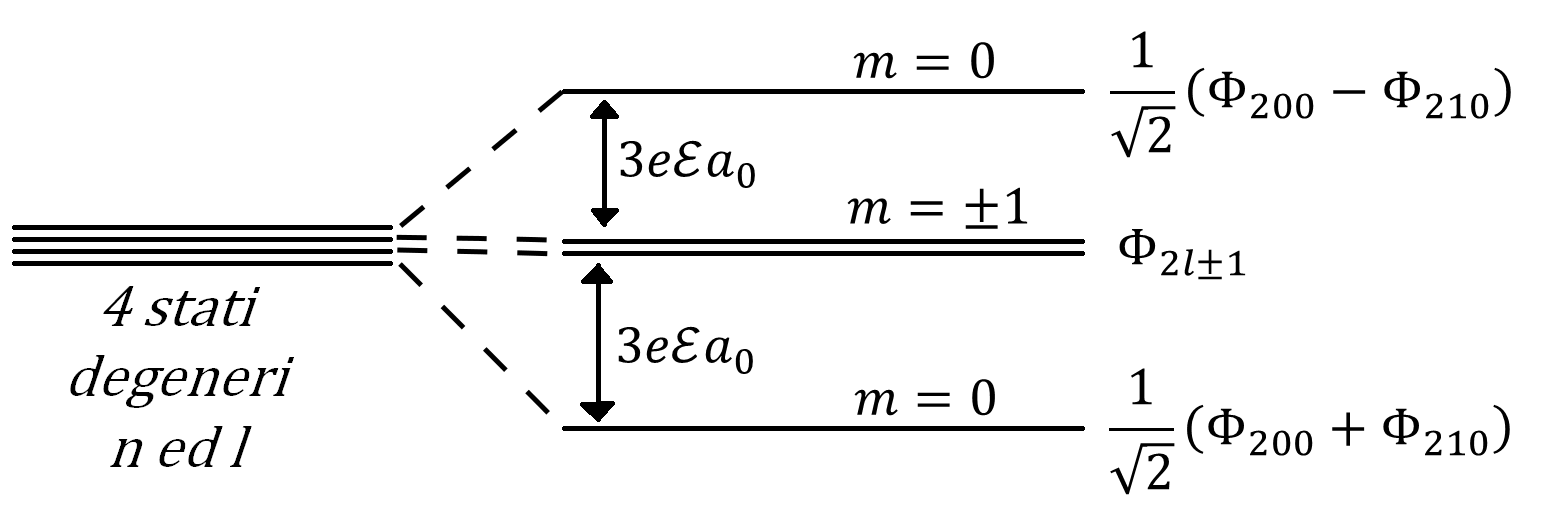
\includegraphics[width=10cm]{immagini/cap_23/fig23_1.png}
\end{center}
Poiché lo spostamento dei livelli, in prima approssimazione, è proporzionale al campo elettrico esterno $\mathcal{E}$, si parla in questo caso di $\textbf{effetto Stark lineare}$.\\
Osserviamo che, \textbf{in presenza del campo elettrico, gli autostati dell'hamiltoniana non sono più autostati di $\boldsymbol{L^2}$}. Ad esempio, nel sottospazio degli stati con $n=2$, abbiamo ottenuto combinazioni lineari di stati corrispondenti ad $l=0$ ed $l=1$. La ragione è che, in presenza del campo elettrico esterno, \textbf{il sistema non è più invariante per rotazioni arbitrarie, e l'hamiltoniana non commuta più con l'operatore momento angolare $\boldsymbol{L^2}$}.\\
Tuttavia, \textbf{il sistema è ancora invariante per rotazione attorno all'asse $\boldsymbol{z}$, che definisce la direzione del campo esterno. L'hamiltoniana perturbata commuta con la proiezione $\boldsymbol{L_z}$ del momento angolare orbitale e gli autostati di $\boldsymbol{H}$ sono simultaneamente autostati di $\boldsymbol{L_z}$}.
\end{document}


